\chapter{Complete Benchmark Topology Panels}\label{app:complete-results}

Chapter~\ref{ch:m-results} uses representative topologies so that all measured backends remain legible. This appendix provides the remaining topology panels generated from the same reconciled allocation-level summaries. It introduces no additional measurements or statistical treatment. Ping-pong is omitted because its complete topology set, \texttt{1n2g} and \texttt{2n1g}, already appears in Figure~\ref{fig:m-pingpong-regimes}.

\section{Halo Exchange}

Figures~\ref{fig:app-halo-isolated} and~\ref{fig:app-halo-steady} separate the single-exchange and 100-exchange contracts. Payload counts two sends and two receives. The multi-node NVSHMEM panels retain the CPU-proxy-assisted \texttt{ibrc} path.

\begin{figure}[htbp]
\centering
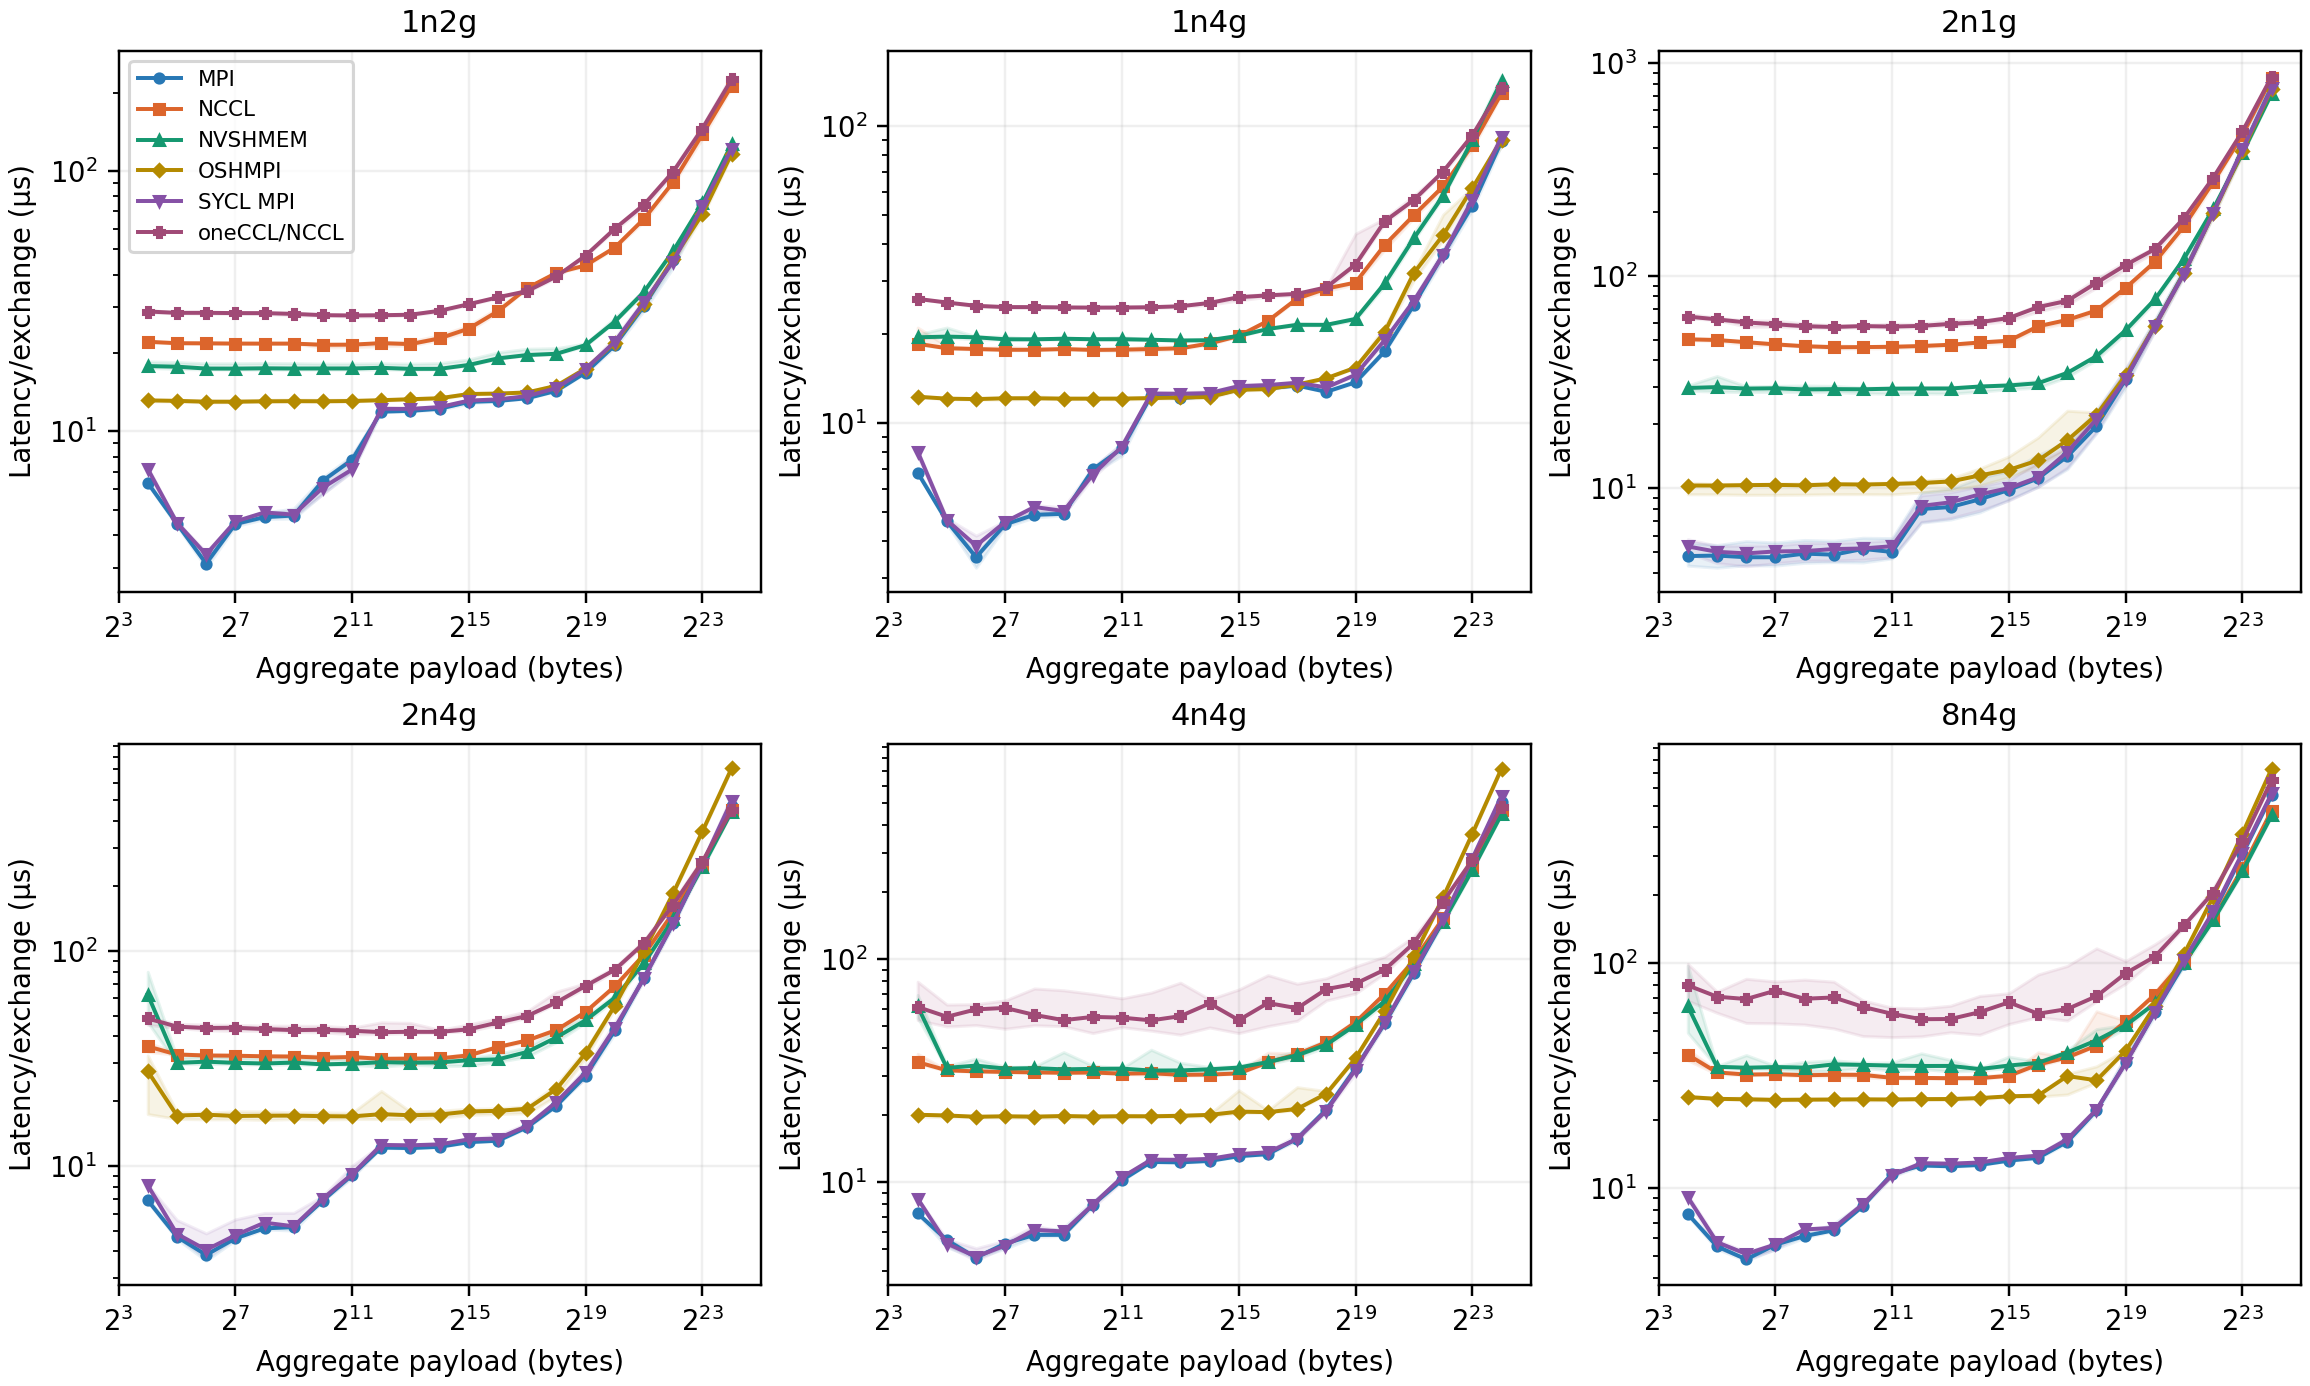
\includegraphics[width=\textwidth]{figures/results/halo-isolated-all-topologies.png}
\caption{Isolated halo latency for all six measured stacks and all six non-single-rank topologies.}
\label{fig:app-halo-isolated}
\end{figure}

\begin{figure}[htbp]
\centering
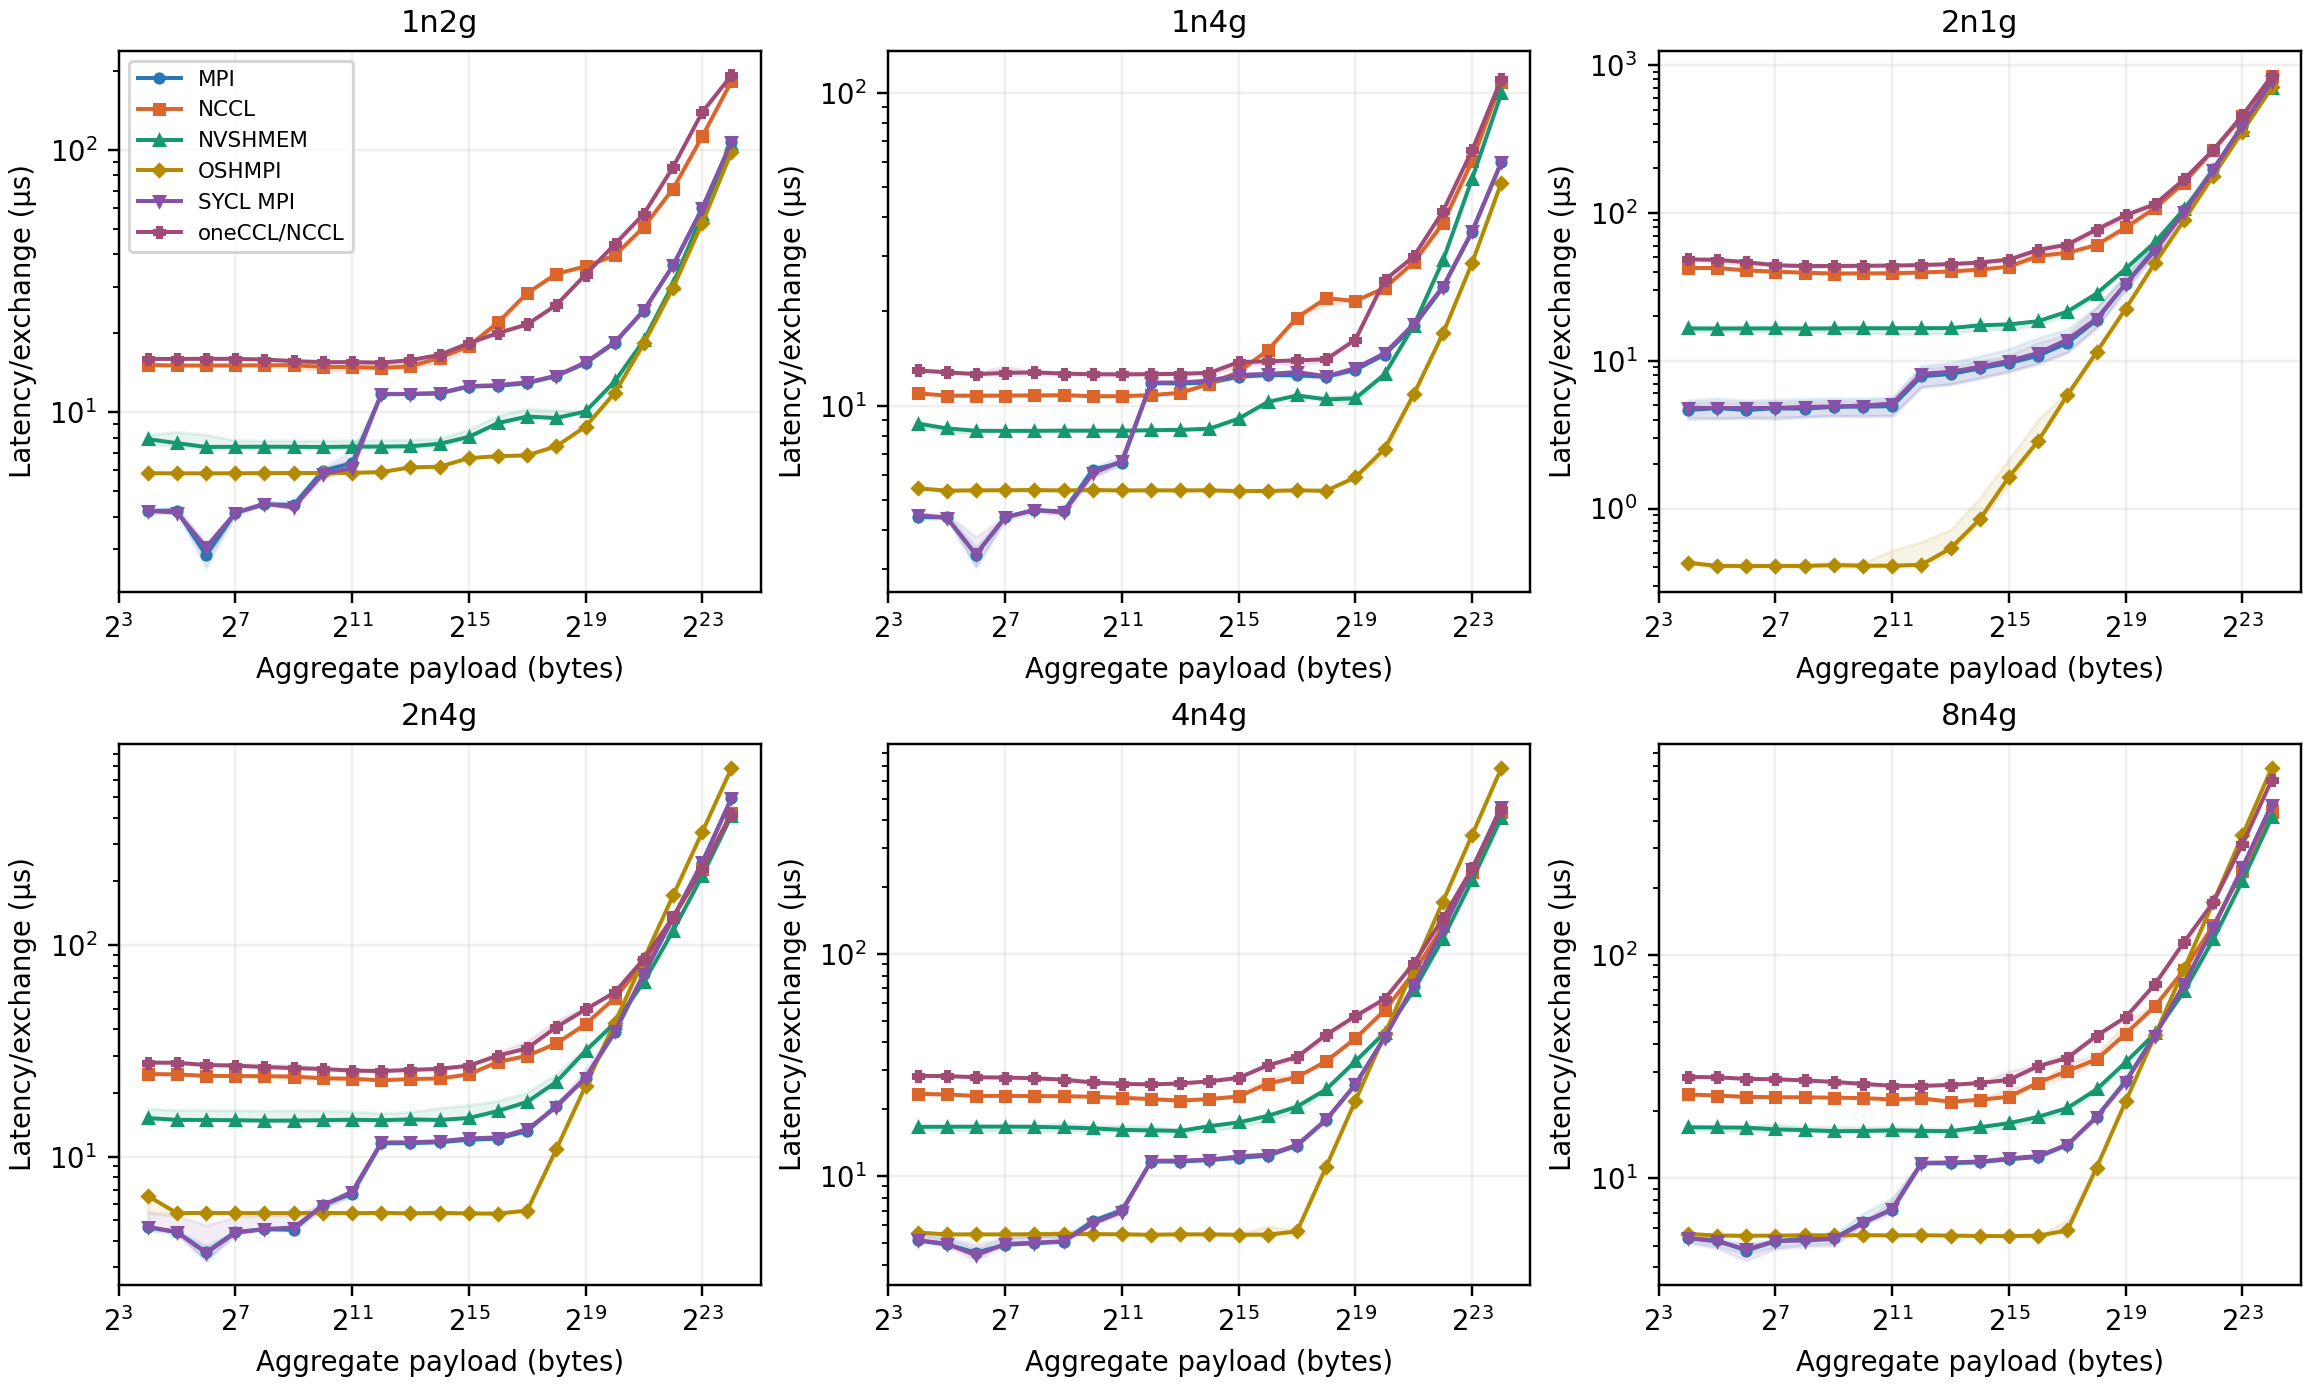
\includegraphics[width=\textwidth]{figures/results/halo-steady-all-topologies.png}
\caption{Steady-state halo latency for all six measured stacks and all six non-single-rank topologies. Values are amortized over batches of 100 exchanges.}
\label{fig:app-halo-steady}
\end{figure}

\section{Collectives}

The single-rank collective panels are implementation controls rather than network baselines. Allreduce uses per-rank input bytes. All-to-all uses bytes per peer, correcting the topology-dependent aggregate-buffer axis in the source analysis artifacts.

\begin{figure}[htbp]
\centering
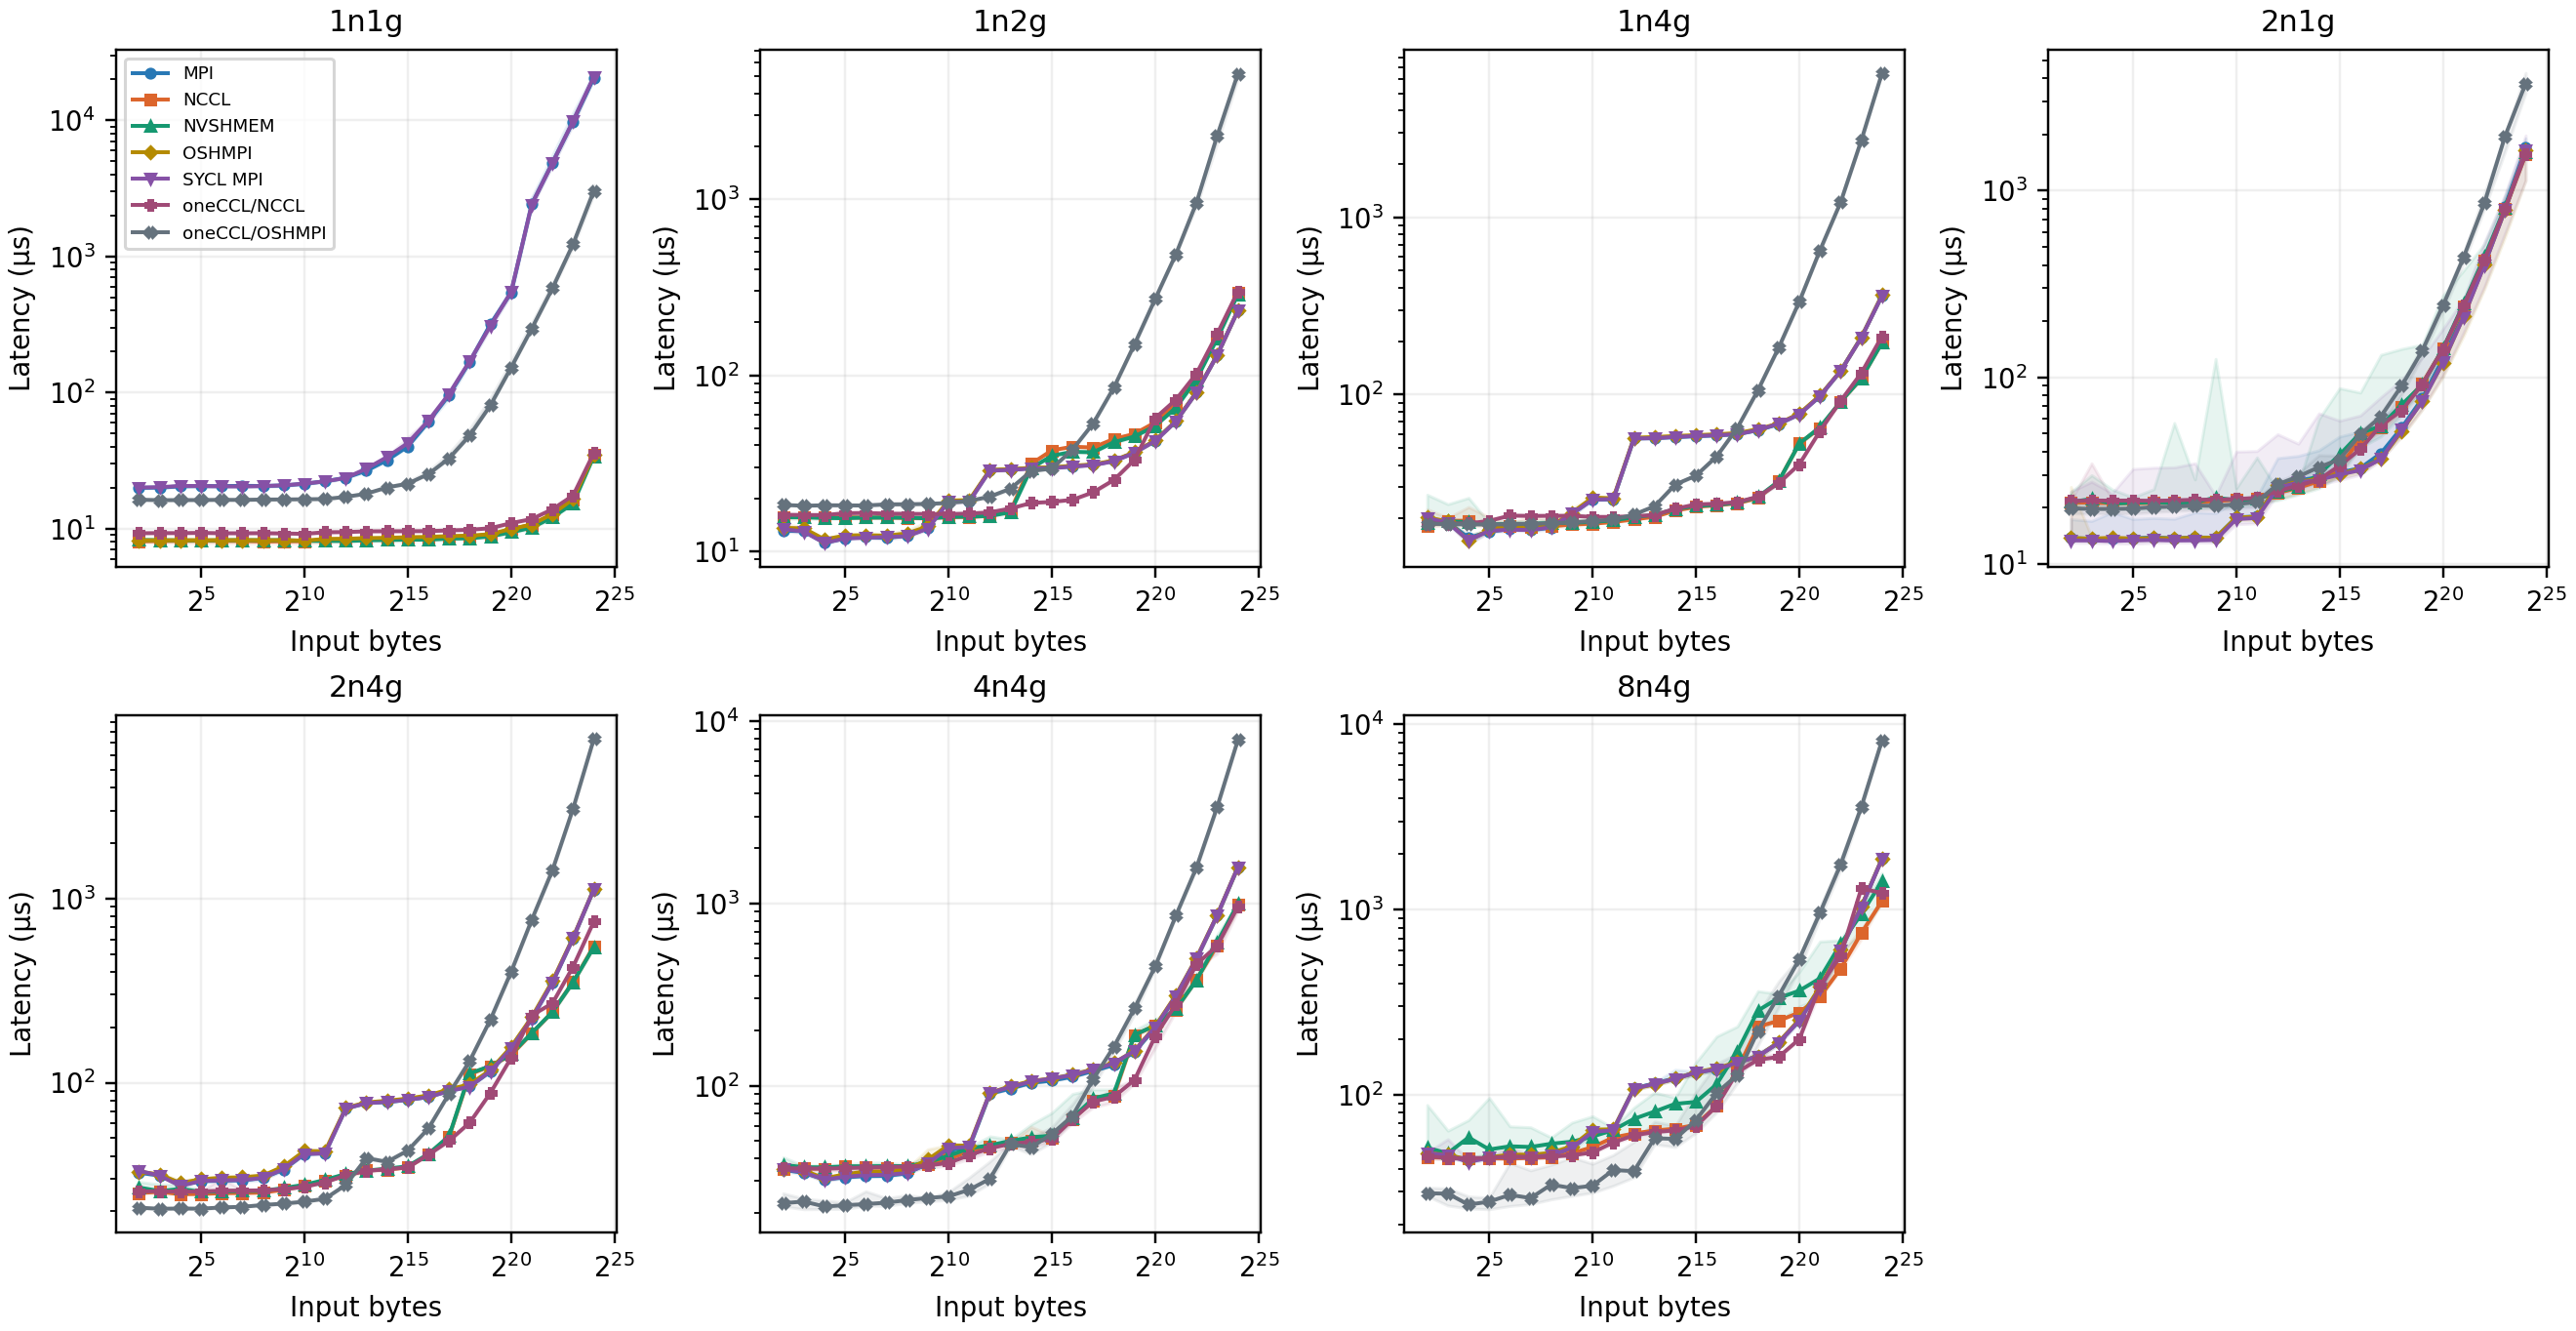
\includegraphics[width=\textwidth]{figures/results/allreduce-all-topologies.png}
\caption{Allreduce latency for all seven measured stacks and all topologies.}
\label{fig:app-allreduce-all}
\end{figure}

\begin{figure}[htbp]
\centering
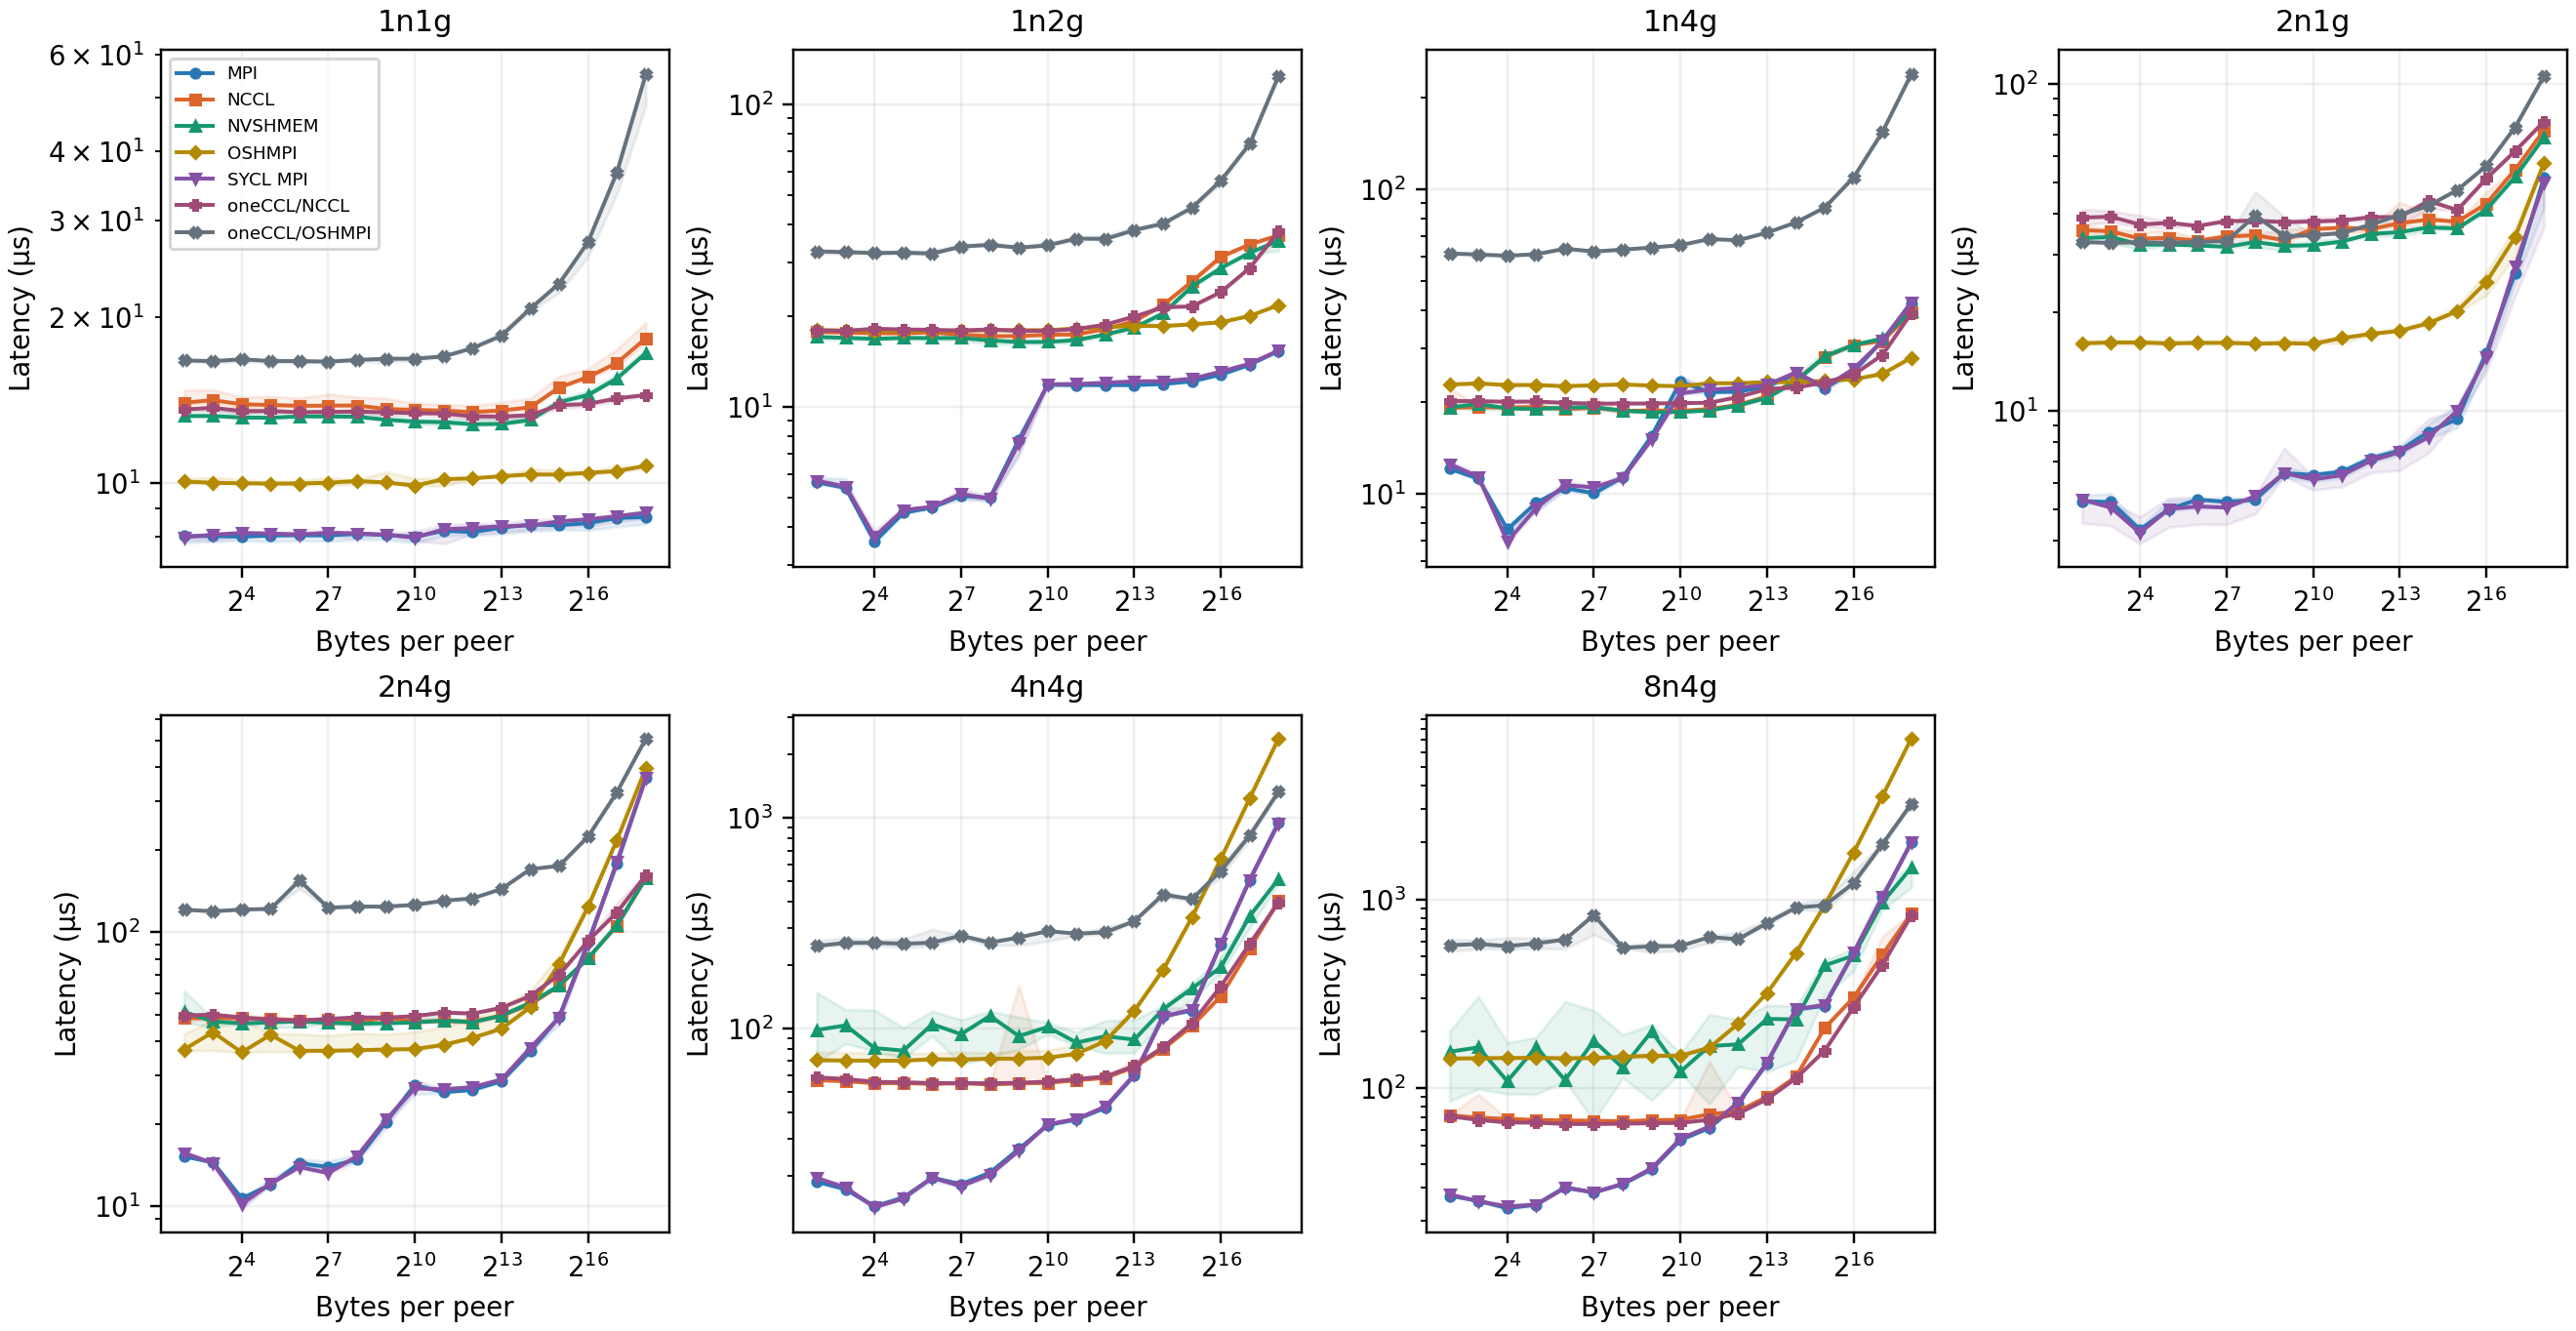
\includegraphics[width=\textwidth]{figures/results/alltoall-all-topologies.png}
\caption{All-to-all latency against bytes per peer for all seven measured stacks and all topologies.}
\label{fig:app-alltoall-all}
\end{figure}

\section{Composite Sequence}

Figure~\ref{fig:app-cg-all} provides every retained \texttt{cg\_step} topology. Ratios use the CUDA MPI median at the same topology and global side as a fixed denominator; the bands do not propagate uncertainty in that denominator. The archived OSHMPI series retains its host-terminal scalar result.

\begin{figure}[htbp]
\centering
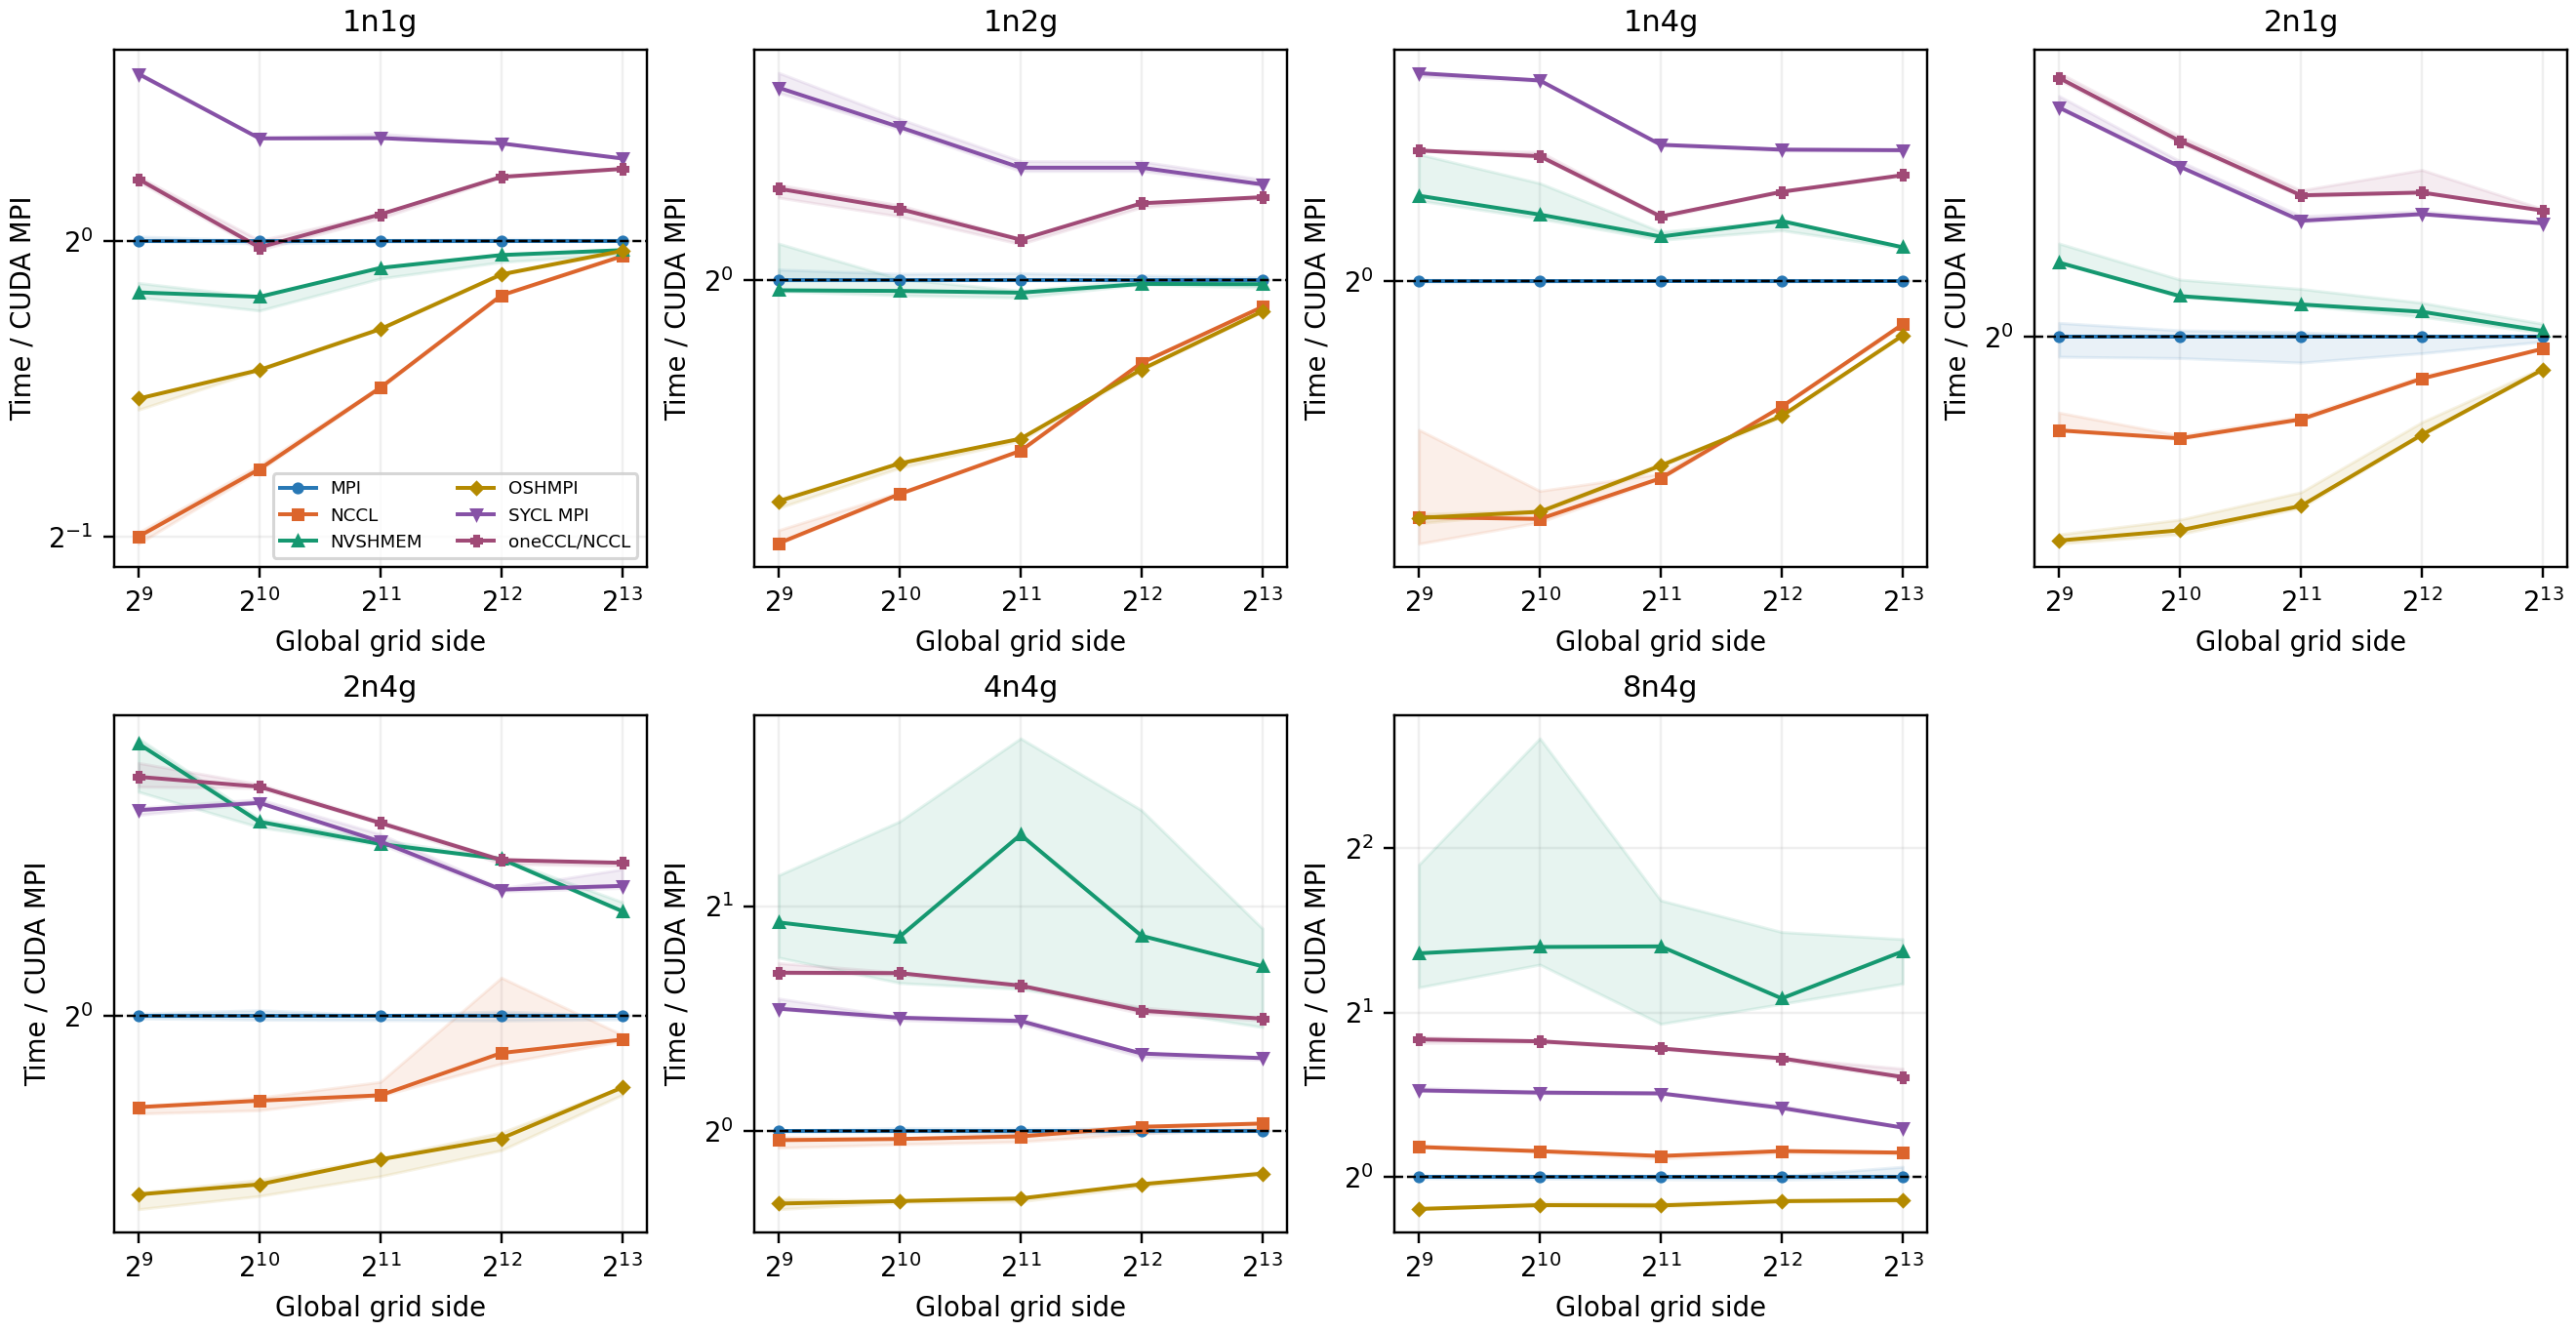
\includegraphics[width=\textwidth]{figures/results/cg-step-all-topologies.png}
\caption{Composite-sequence time relative to CUDA MPI for all six measured stacks and all topologies.}
\label{fig:app-cg-all}
\end{figure}
